\newif\ifshowsolutions
\showsolutionstrue
\documentclass{article}
\usepackage{listings}
\usepackage{amsmath}
%\usepackage{subfigure}
\usepackage{subfig}
\usepackage{amsthm}
\usepackage{amsmath}
\usepackage{amssymb}
\usepackage{graphicx}
\usepackage{mdwlist}
\usepackage[colorlinks=true]{hyperref}
\usepackage{geometry}
\usepackage{titlesec}
\geometry{margin=1in}
\geometry{headheight=2in}
\geometry{top=2in}
\usepackage{palatino}
\usepackage{mathrsfs}
\usepackage{fancyhdr}
\usepackage{paralist}
\usepackage{todonotes}
\setlength{\marginparwidth}{2.15cm}
\usepackage{tikz}
\usetikzlibrary{positioning,shapes,backgrounds}
\usepackage{float} % Place figures where you ACTUALLY want it
\usepackage{comment} % a hack to toggle sections
\usepackage{ifthen}
\usepackage{mdframed}
\usepackage{verbatim}
\usepackage[strings]{underscore}
\usepackage{listings}
\usepackage{bbm}
\rhead{}
\lhead{}

\renewcommand{\baselinestretch}{1.15}

% Shortcuts for commonly used operators
\newcommand{\E}{\mathbb{E}}
\newcommand{\Var}{\operatorname{Var}}
\newcommand{\Cov}{\operatorname{Cov}}
\newcommand{\Bias}{\operatorname{Bias}}
\DeclareMathOperator{\argmin}{arg\,min}
\DeclareMathOperator{\argmax}{arg\,max}

% do not number subsection and below
\setcounter{secnumdepth}{1}

% custom format subsection
\titleformat*{\subsection}{\large\bfseries}

% set up the \question shortcut
\newcounter{question}[section]
\newenvironment{question}[1][]
  {\refstepcounter{question}\par\addvspace{1em}\textbf{Question~\Alph{question}\!
    \ifthenelse{\equal{#1}{}}{}{ [#1 points]}: }}
    {\par\vspace{\baselineskip}}

\newcounter{subquestion}[question]
\newenvironment{subquestion}[1][]
  {\refstepcounter{subquestion}\par\medskip\textbf{\roman{subquestion}.\!
    \ifthenelse{\equal{#1}{}}{}{ [#1 points]:}} }
  {\par\addvspace{\baselineskip}}

\titlespacing\section{0pt}{12pt plus 2pt minus 2pt}{0pt plus 2pt minus 2pt}
\titlespacing\subsection{0pt}{12pt plus 4pt minus 2pt}{0pt plus 2pt minus 2pt}
\titlespacing\subsubsection{0pt}{12pt plus 4pt minus 2pt}{0pt plus 2pt minus 2pt}


\newenvironment{hint}[1][]
  {\begin{em}\textbf{Hint: }}{\end{em}}

\ifshowsolutions
  \newenvironment{solution}[1][]
    {\par\medskip \begin{mdframed}\textbf{Solution~\Alph{question}#1:} \begin{em}}
    {\end{em}\medskip\end{mdframed}\medskip}
  \newenvironment{subsolution}[1][]
    {\par\medskip \begin{mdframed}\textbf{Solution~\Alph{question}#1.\roman{subquestion}:} \begin{em}}
    {\end{em}\medskip\end{mdframed}\medskip}
\else
  \excludecomment{solution}
  \excludecomment{subsolution}
\fi

\newcommand{\boldline}[1]{\underline{\textbf{#1}}}

\chead{%
  {\vbox{%
      \vspace{2mm}
      \large
      Machine Learning \& Data Mining \hfill
      Caltech CS/CNS/EE 155 \hfill \\[1pt]
      Miniproject 3\hfill
      March $11^{th}$, 2017 \\
    }
  }
}

\begin{document}
\pagestyle{fancy}

% LaTeX is simple if you have a good template to work with! To use this document, simply fill in your text where we have indicated. To write mathematical notation in a fancy style, just write the notation inside enclosing $dollar signs$.

% For example:
% $y = x^2 + 2x + 1$

% For help with LaTeX, please feel free to see a TA!


\pagebreak
\section{Introduction}
\medskip
\begin{itemize}

    \item \boldline{Group members} \\
    Bolton Bailey and David Inglis

    \item \boldline{Team name} \\
    One Hot Team

    \item \boldline{Division of labour} \\
    We both pair coded the  visualization generators and discussed how to approach the project together.

\end{itemize}


\pagebreak
\section{Basic Visualizations}
\medskip



\begin{figure}[H]
\centering
\includegraphics[width=\textwidth]{all_ratings_bar_chart}
\caption{Visualization of ratings for all movies in the dataset.}
\end{figure}


\pagebreak

\begin{figure}[H]
\centering
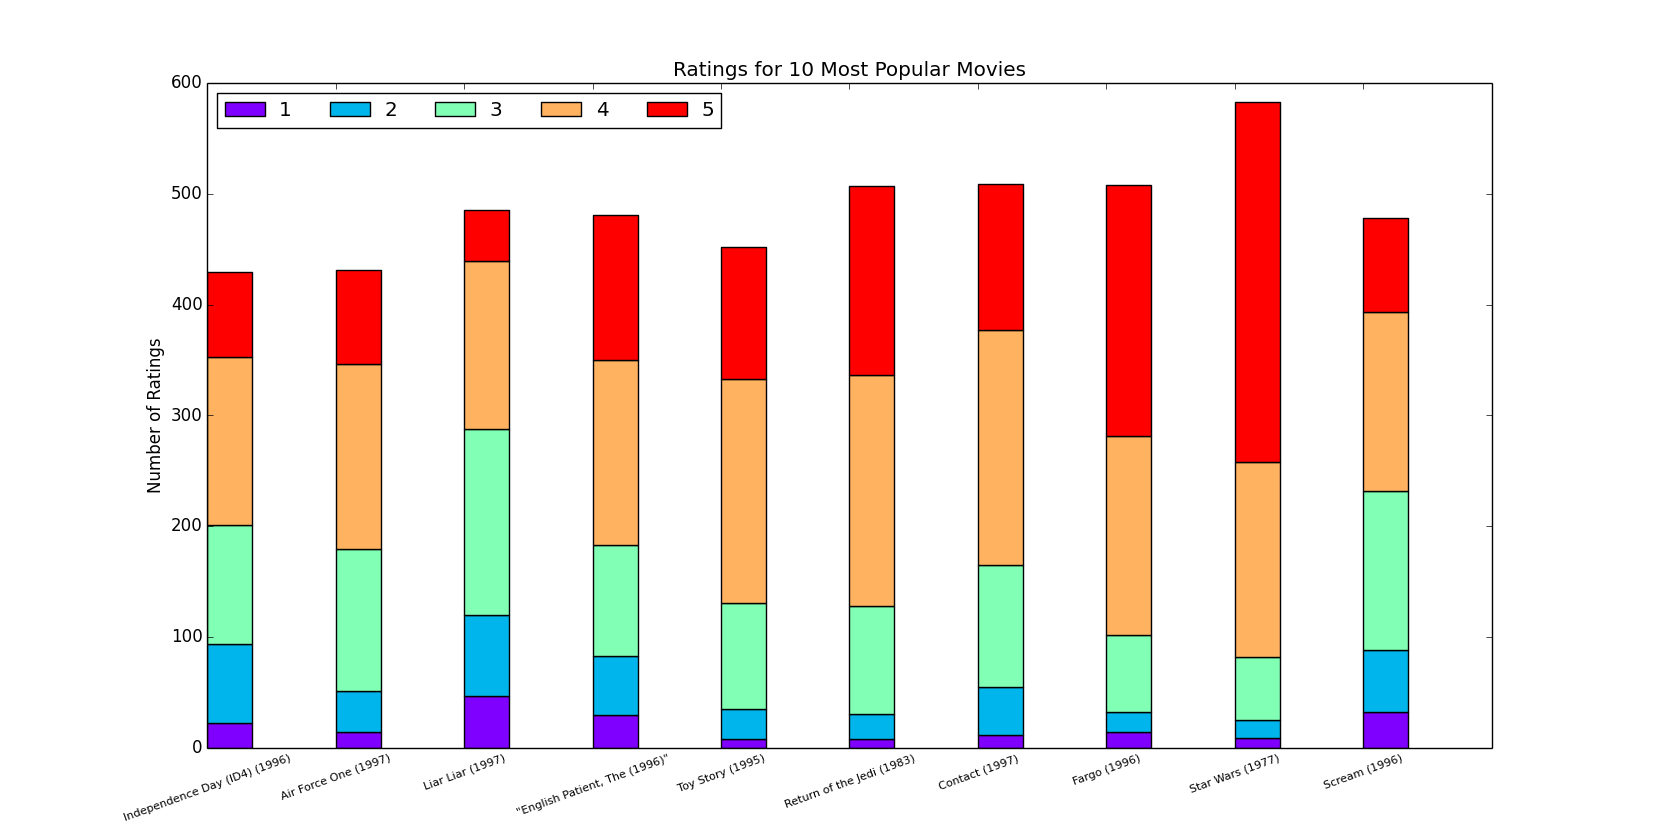
\includegraphics[width=\textwidth]{most-popular}
\caption{Visualization of ratings for most popular movies in the dataset.}
\end{figure}

\pagebreak

\begin{figure}[H]
\centering
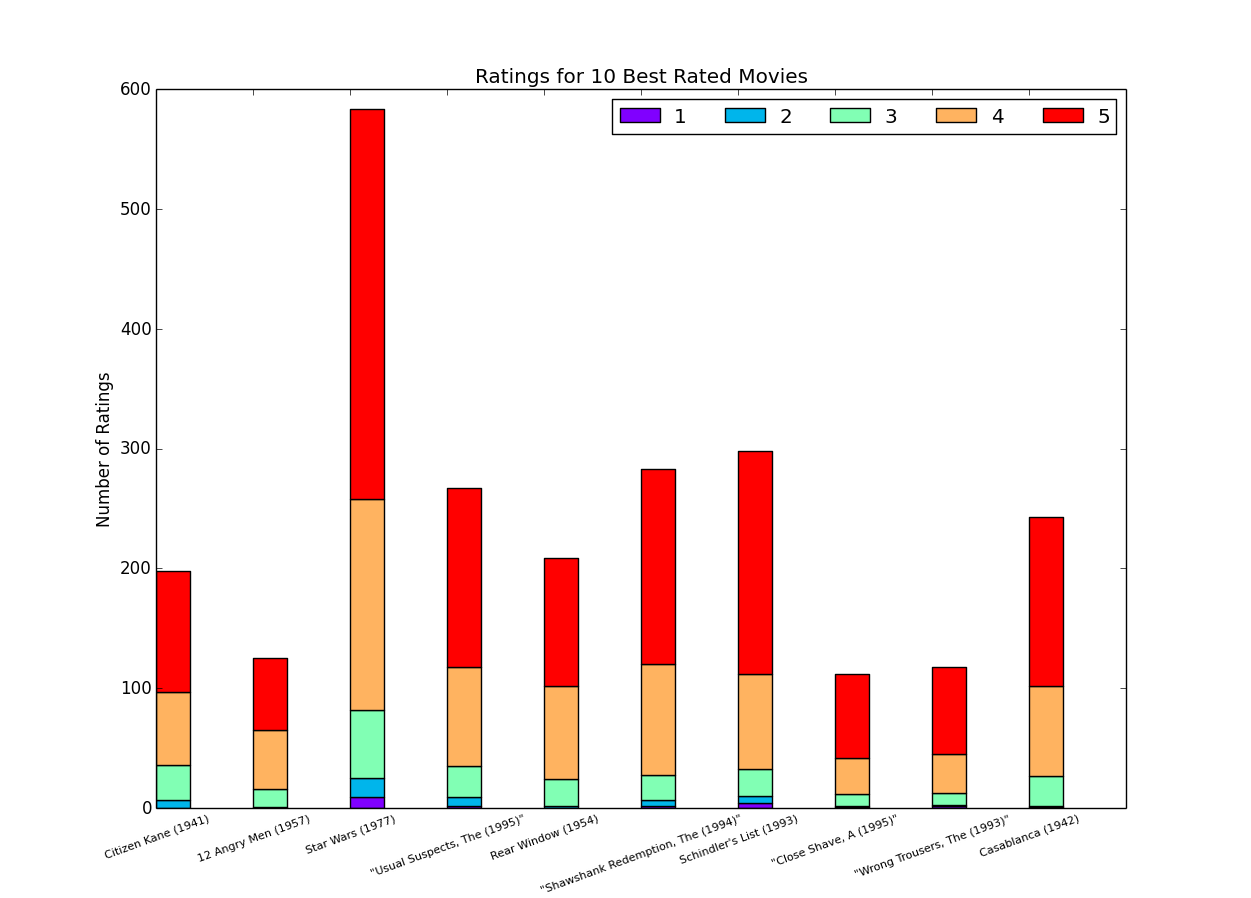
\includegraphics[width=\textwidth]{best-rated}
\caption{Visualization of ratings for best rated movies in the dataset.}
\end{figure}

\pagebreak

\begin{figure}[H]
\centering
\includegraphics[width=\textwidth]{Crime_ratings_bar_chart}
\caption{Visualization of ratings for all Crime movies in the dataset.}
\end{figure}

\pagebreak

\begin{figure}[H]
\centering
\includegraphics[width=\textwidth]{Documentary_ratings_bar_chart}
\caption{Visualization of ratings for all Documentary movies in the dataset.}
\end{figure}


\pagebreak

\begin{figure}[H]
\centering
\includegraphics[width=\textwidth]{Fantasy_ratings_bar_chart}
\caption{Visualization of ratings for all Fantasy movies in the dataset.}
\end{figure}

\begin{itemize}


    \item \boldline{Justify your choice of visualization method}
    \begin{itemize}
    % Insert text here. Bullet points can be made using '\item'. Models and techniques should be bolded using '\textbf{}'.
    \item \textbf{All ratings in the MovieLens Dataset:} To display all ratings in the MovieLens dataset, we decided it would be best to use a bar chart, with one bar for the number of 1 ratings, one bar for the number of 2 ratings, and so on up to 5. Since the data we needed to show was just t\pagebreakhe relative number of ratings of each level, we felt that this visualization would be the simplest and most effective

    \item \textbf{All ratings of the ten most popular movies:} To display the most popular movies ratings in the MovieLens dataset, we created a stacked bar chart. We placed the ten most popular movies along the x-axis, and then created a bar for each of these, for which th total height of the bar represented the total number of ratings, and each bar had different portions colored differently to show what proportion of the ratings were 1, what proportion were 2 and so on. We felt that this format allowed the chart to simulataneously convey the total number of ratings for each movie, as well as how positive in general those ratings were.

    \item \textbf{All ratings of the ten best movies:} To display the best movies ratings in the MovieLens dataset, we created a stacked bar chart. Again, we felt that this format allowed the chart to simulataneously convey the total number of ratings for each movie, as well as how positive in general those ratings were. We also felt it would be good to be able to compare this chart to the most popular movies chart. We also chose to disqualify all movies rated less than 100 times, since it could be possible to have a movie which is generally unliked, but which only a few people rated and which was rated highly by all who rated it.

    \item \textbf{All ratings of movies from three genres of your choice:} To display all ratings for the three specific genres we chose (Crime, Documentary, and Fantasy), we used a bar chart with one bar for each value for the ratings, like we used for the set of all movies. We felt that this would allow us to see how well-liked and also how polarizing genres were with respect to others and with respect to the dataset as a whole.

    \end{itemize}

    \item \boldline{Observations}
    \begin{itemize}
    % Insert text here. Bullet points can be made using '\item'.
    \item \textbf{All ratings in the MovieLens Dataset:} In the bar chart we created for all ratings, we can see a bell-curve shape. The most common rating is 4, and ratings further away from 4 get less and less common. We expected to see this, as we feel that most movies are ok, and there are a few exceptionally good movies, and a few bad movies.

    \item \textbf{All ratings of the ten most popular movies:} In the stacked bar chart for the ratings for the ten most popular movies, we can see that these movies were all rated around 500 times. We can see that these movies were commonly rated 4, except for Star Wars, which was very well-liked, and had a lot of 5 ratings. Overall, we expected the more-often ranked movies to be better rated than we saw, because we thought bad movies probably wouldn't be watched as much. However, 1 ratings were very uncommon, so maybe it is only the very very bad movies which are rarely watched.

    \item \textbf{All ratings of the ten best movies:} In the stacked bar chart for the ratings for the ten most well-liked movies, we can see that these movies were less frequently rated, usually around 200 times. In contrast to the most popular movies, and in accordance with our expecatations, these movies were rated 5 overwhelmingly often.

    \item \textbf{All ratings of movies from three genres of your choice:} In the bar charts for the three specific genres we chose (Crime, Documentary, and Fantasy), we see similar trends to the data as a whole: All three are unimodal. We note that there are fewer Documentaries, but that low ratings for documentaries are very uncommon, indicating that bad documentaries are rare. We also note that the mode of the Fantasy genre rating was 3: It seems that fantasy movies aren't as well-liked.

    \end{itemize}



\end{itemize}


\pagebreak
\section{Matrix Factorization Algorithm}
\medskip
\begin{itemize}

    \item \boldline{Overall Implementation Architecture}
    We used the TA-provided HW6 solution for the matrix factorization portion. Once
    we had our factored matrix, we used numpy's implementation of single value decomposition
    to reduce the dimensionality of the data down to 2 dimensions.

    \item \boldline{What parameters did you adjust and how?} \\

    \begin{itemize}
    \item \textbf{Stopping Criteria:} The default TA implementation of matrix factorization performs stochastic
    gradient descent until the difference in mean-squared error between two
    consecutive epochs is less than some $\epsilon$ fraction of the initial
    decrease in error from the start state to the first epoch. We experimented
    with varying val\pagebreakues for this epsilon, ranging from $10e-4$ by several factors of
    $10$ in either direction, but found that unless we chose a very
    large $\epsilon$ the model converged to pretty much the same thing every time,
    so it didn't really matter what we chose. Using the default value, $\epsilon = 10e-4$,
    there was not much variation in results from run to run, so we decided to stick
    with that.

    \item \textbf{Step Size:} The step size shouldn't really affect what the
    gradient descent converges to, unless it is so big that it causes the descent
    to oscillate and diverge. The only disadvantage to choosing a very small
    $\eta$ is that the SGD procedure will take longer to converge. We chose
    $\eta = 0.03$ which converged in a reasonable number of iterations, while
    providing the same level of accuracy as smaller $\eta$ values.

    \item \textbf{Regularization Parameter:} This was the value we experimented
    the most with. A larger $\lambda$ value will regularize the data more and bias
    the output matrices towards simpler models, while a lower $\lambda$ value leads
    to a more complex, unconstrained solution. We experimented with the following
    $\lambda$ values: $0$, $0.001$, $0.01$, $0.1$, and $1$. For the same set of
    movies, $\lambda = 0.001$ provided the most easily interpreted results, so
    we chose to use that $\lambda$ value.
    \end{itemize}

    \item \boldline{Did you make any other significant modifications or additions?} \\

    Besides the parameter tuning mentioned above we stuck to the stock TA and numpy
    implementations of matrix factorization and single value decomposition.
\end{itemize}


\pagebreak
\section{Matrix Factorization Visualization}
\medskip

\begin{figure}[H]
\centering
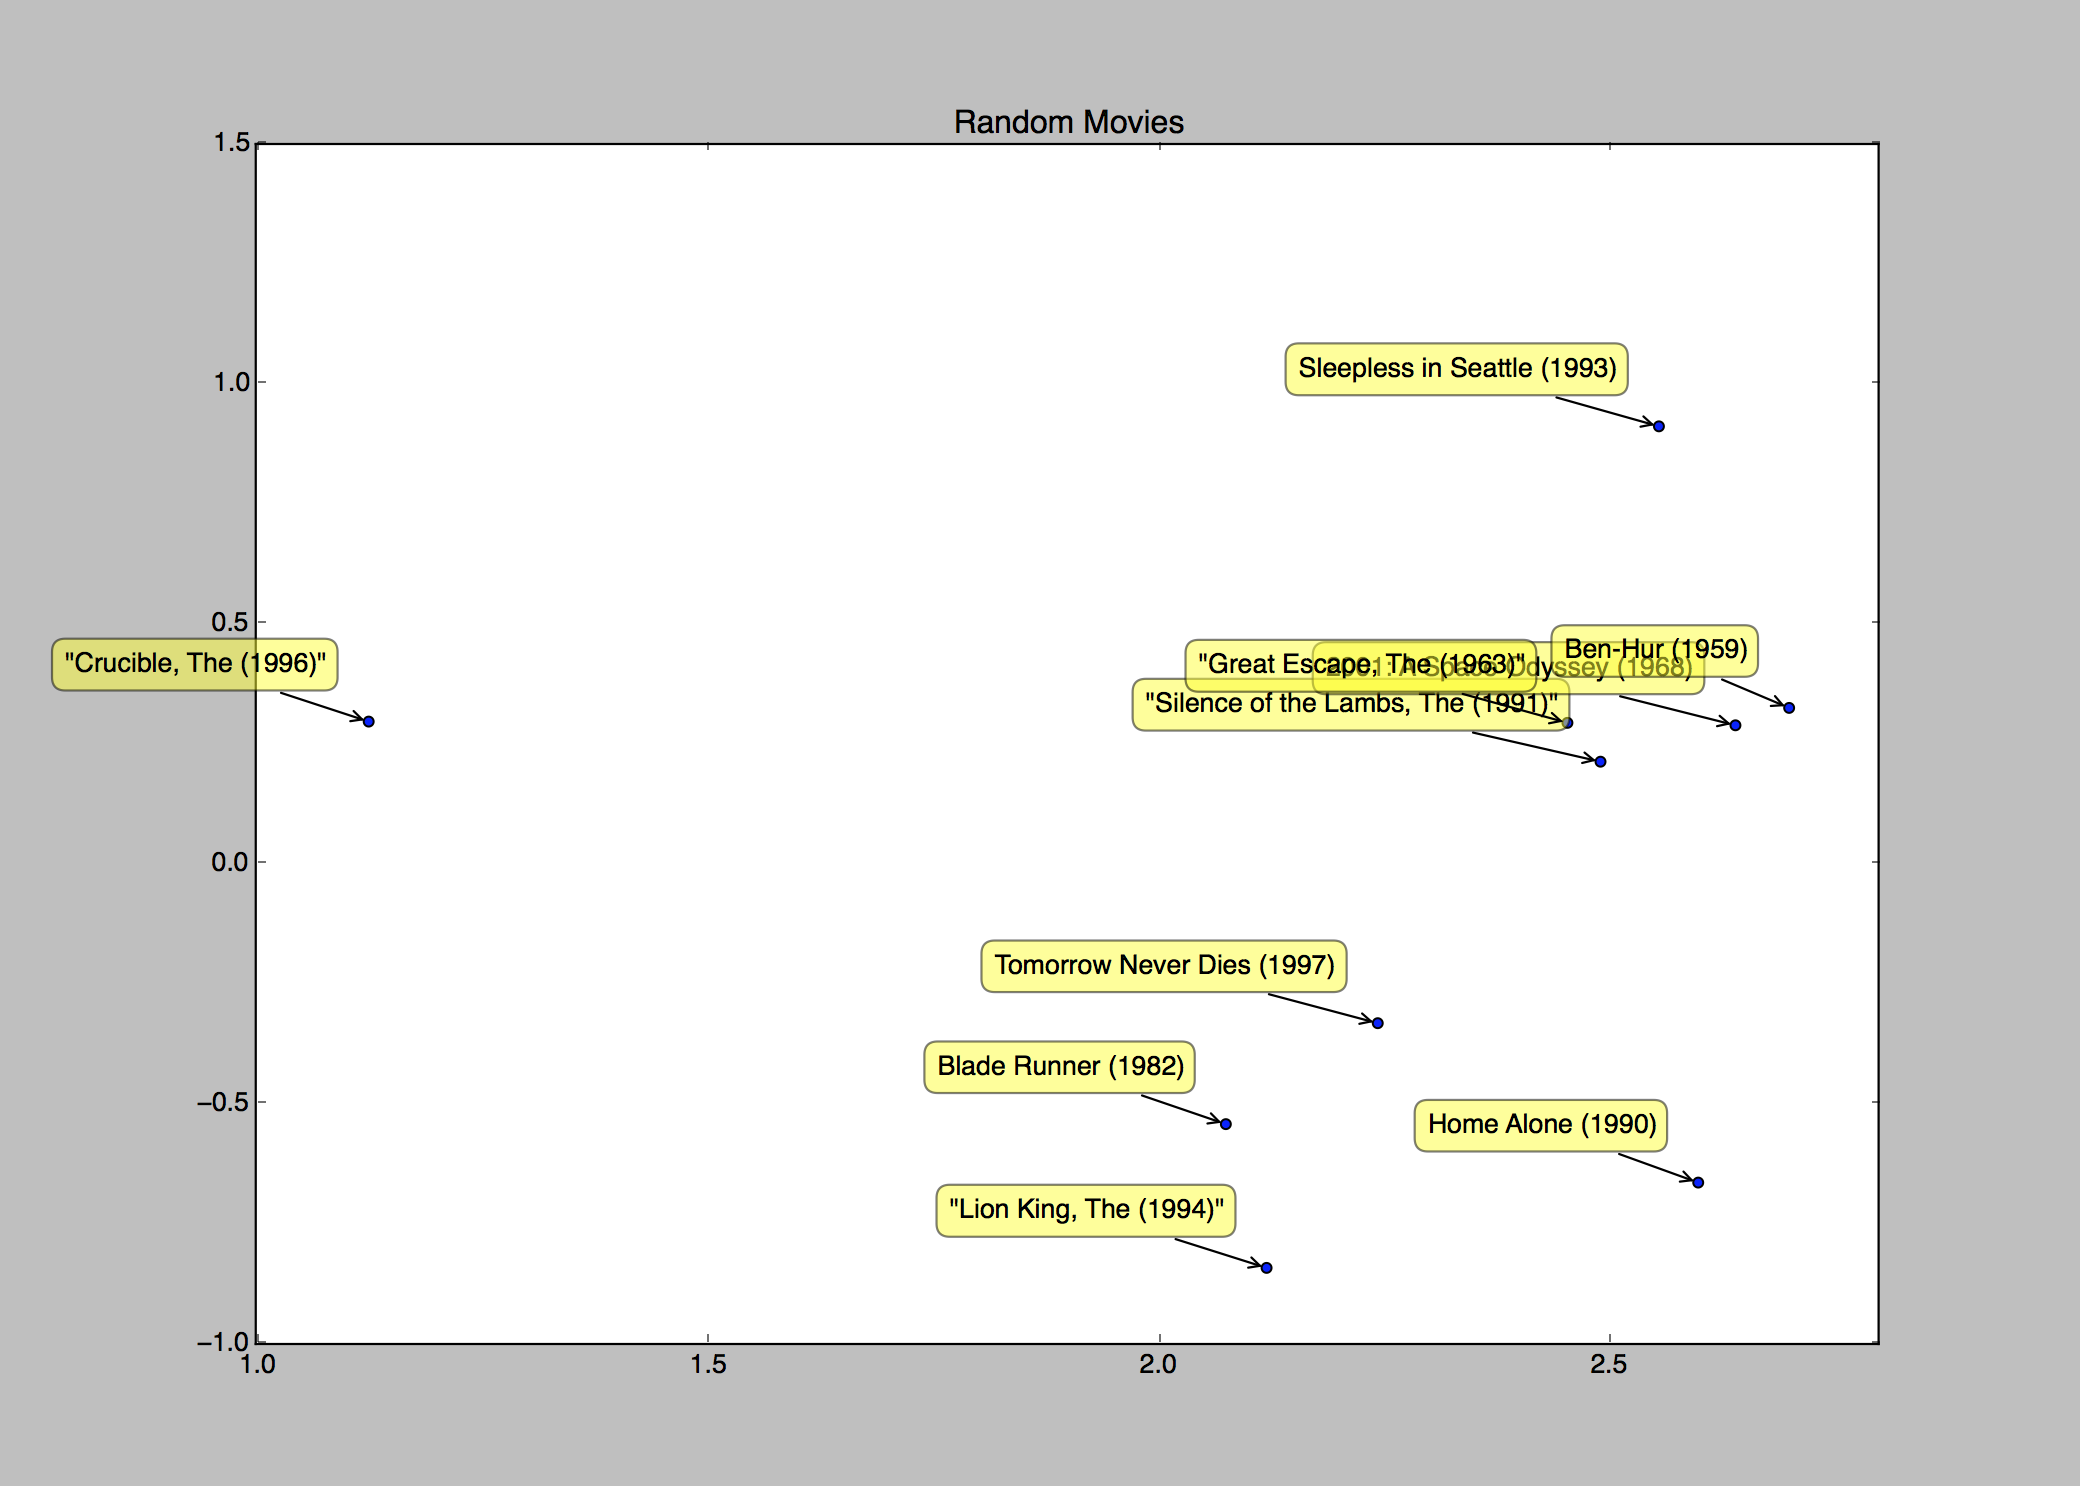
\includegraphics[width=\textwidth]{random_2d_vis}
\caption{2D visualization of parameters for 10 random movies in the dataset.}
\end{figure}


\pagebreak

\begin{figure}[H]
\centering
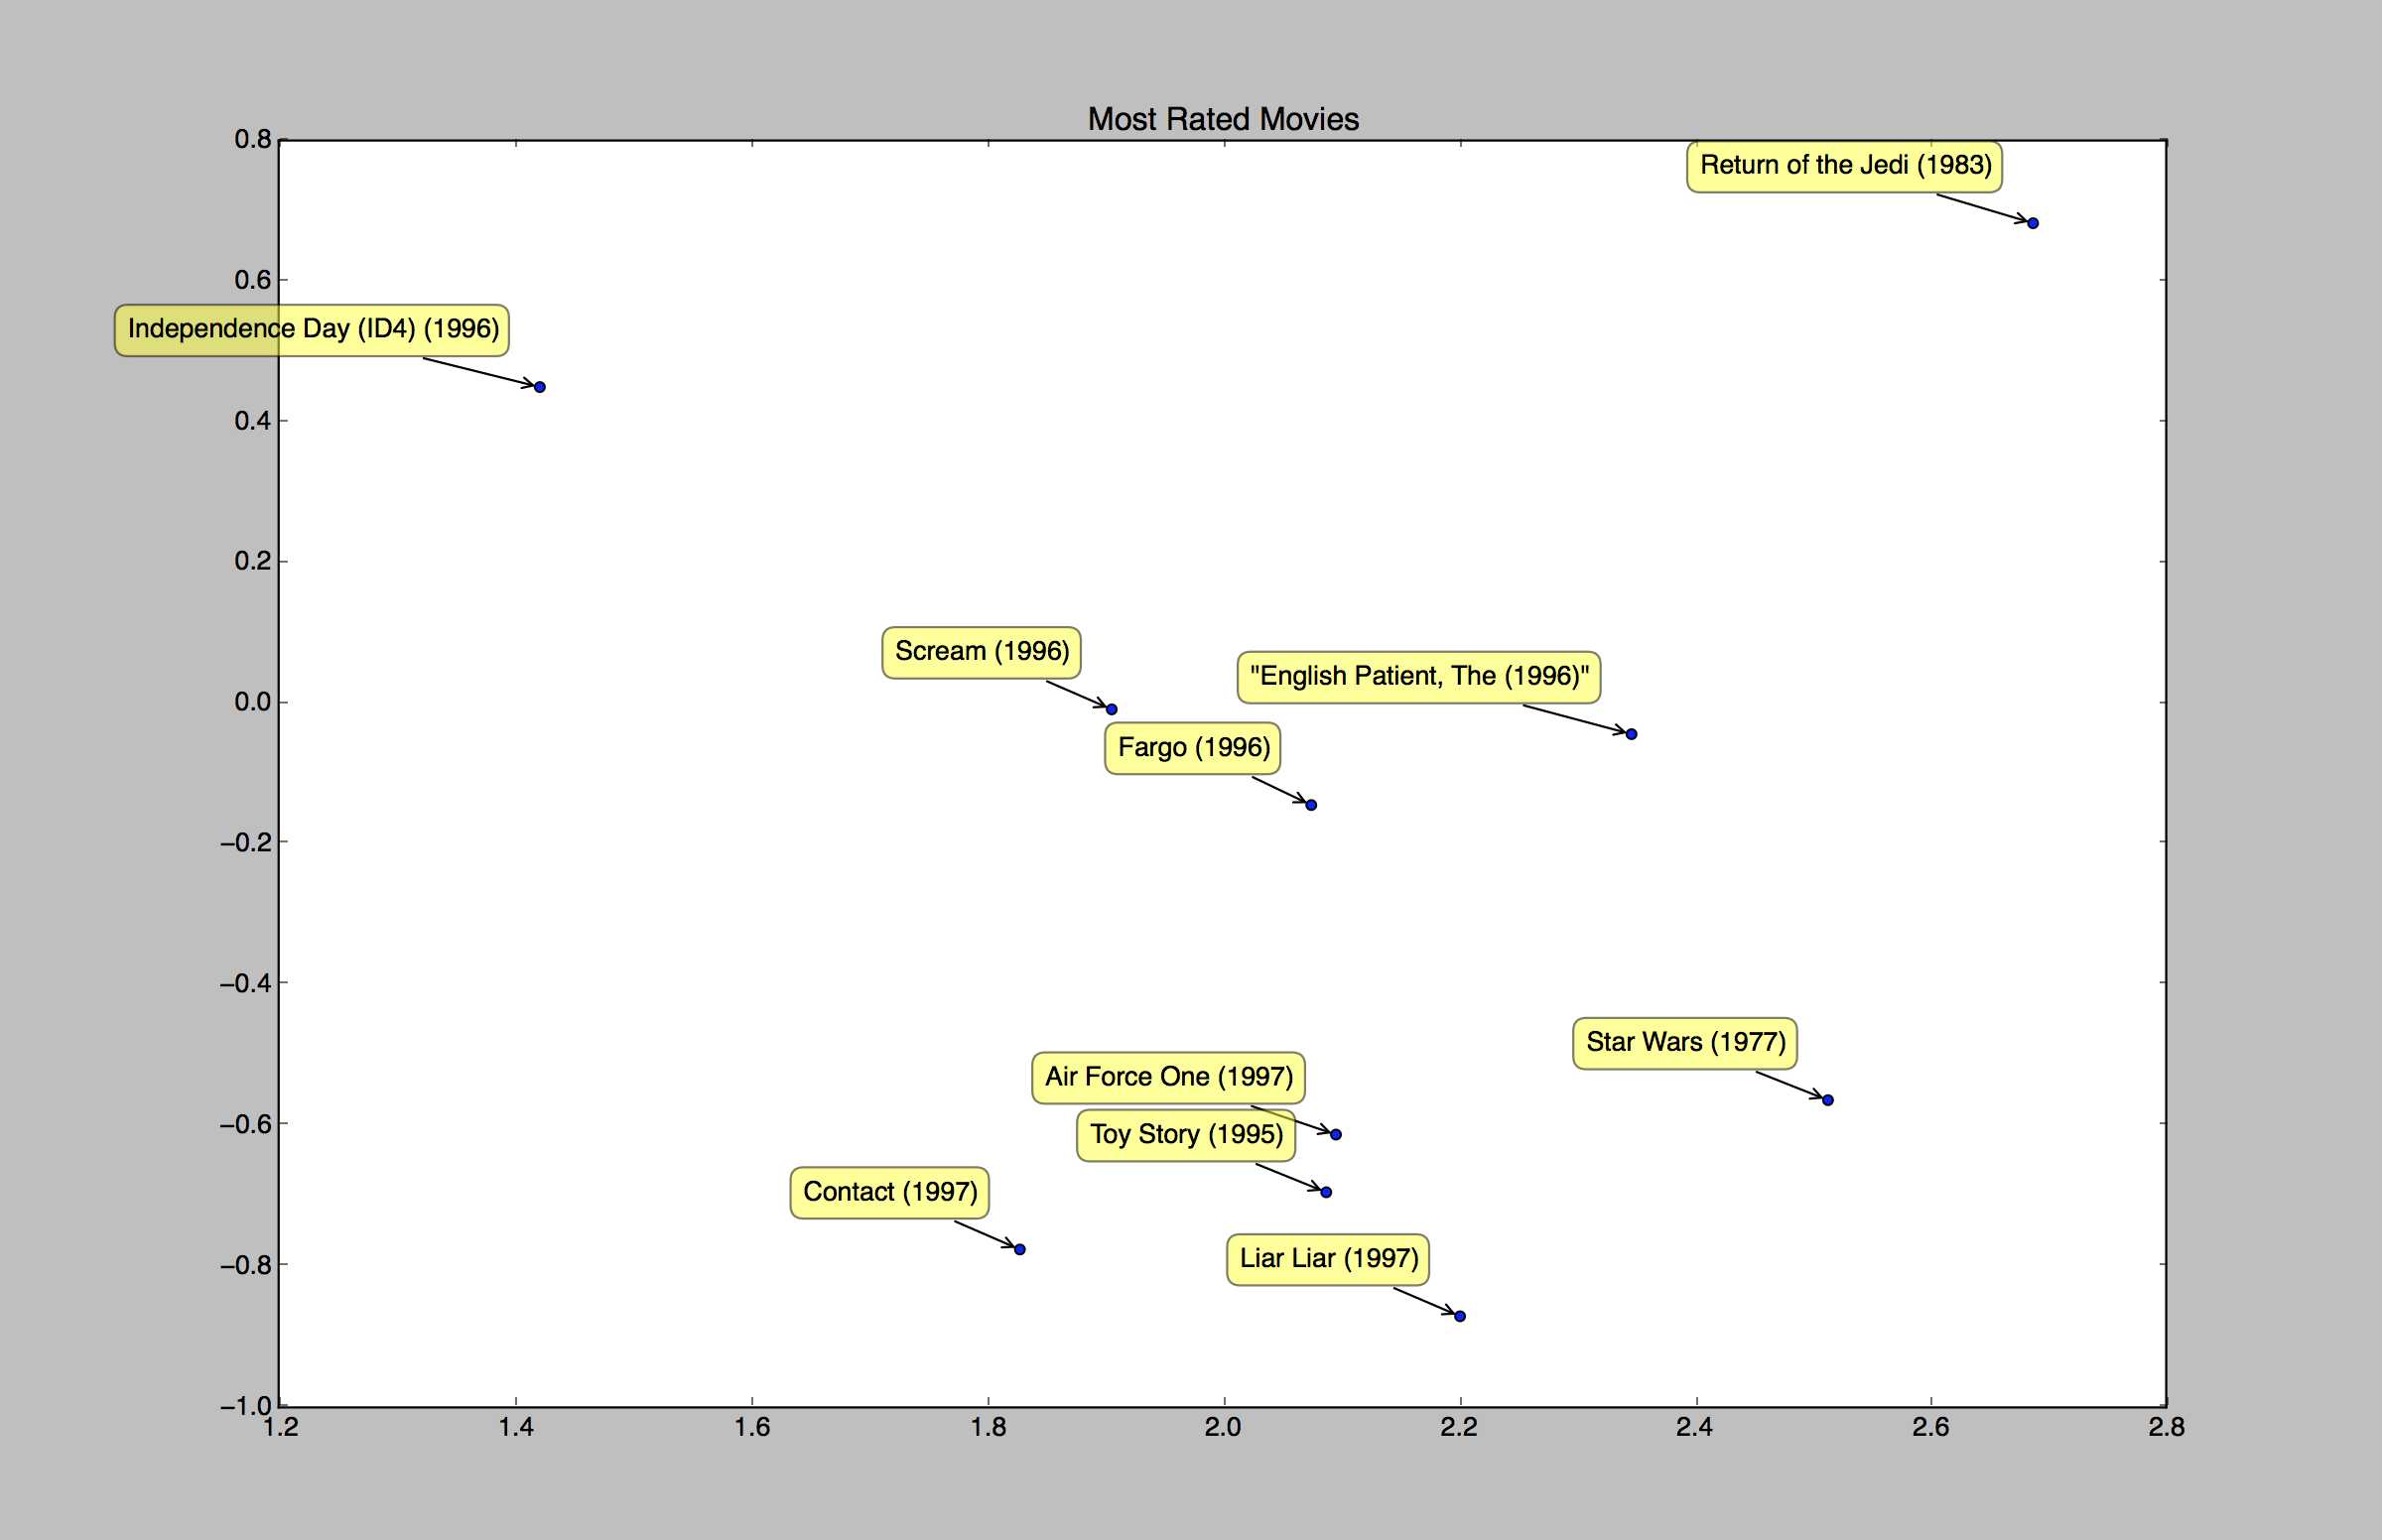
\includegraphics[width=\textwidth]{popular_2d_vis}
\caption{2D visualization of parameters for 10 most popular movies in the dataset.}
\end{figure}


\pagebreak

\begin{figure}[H]
\centering
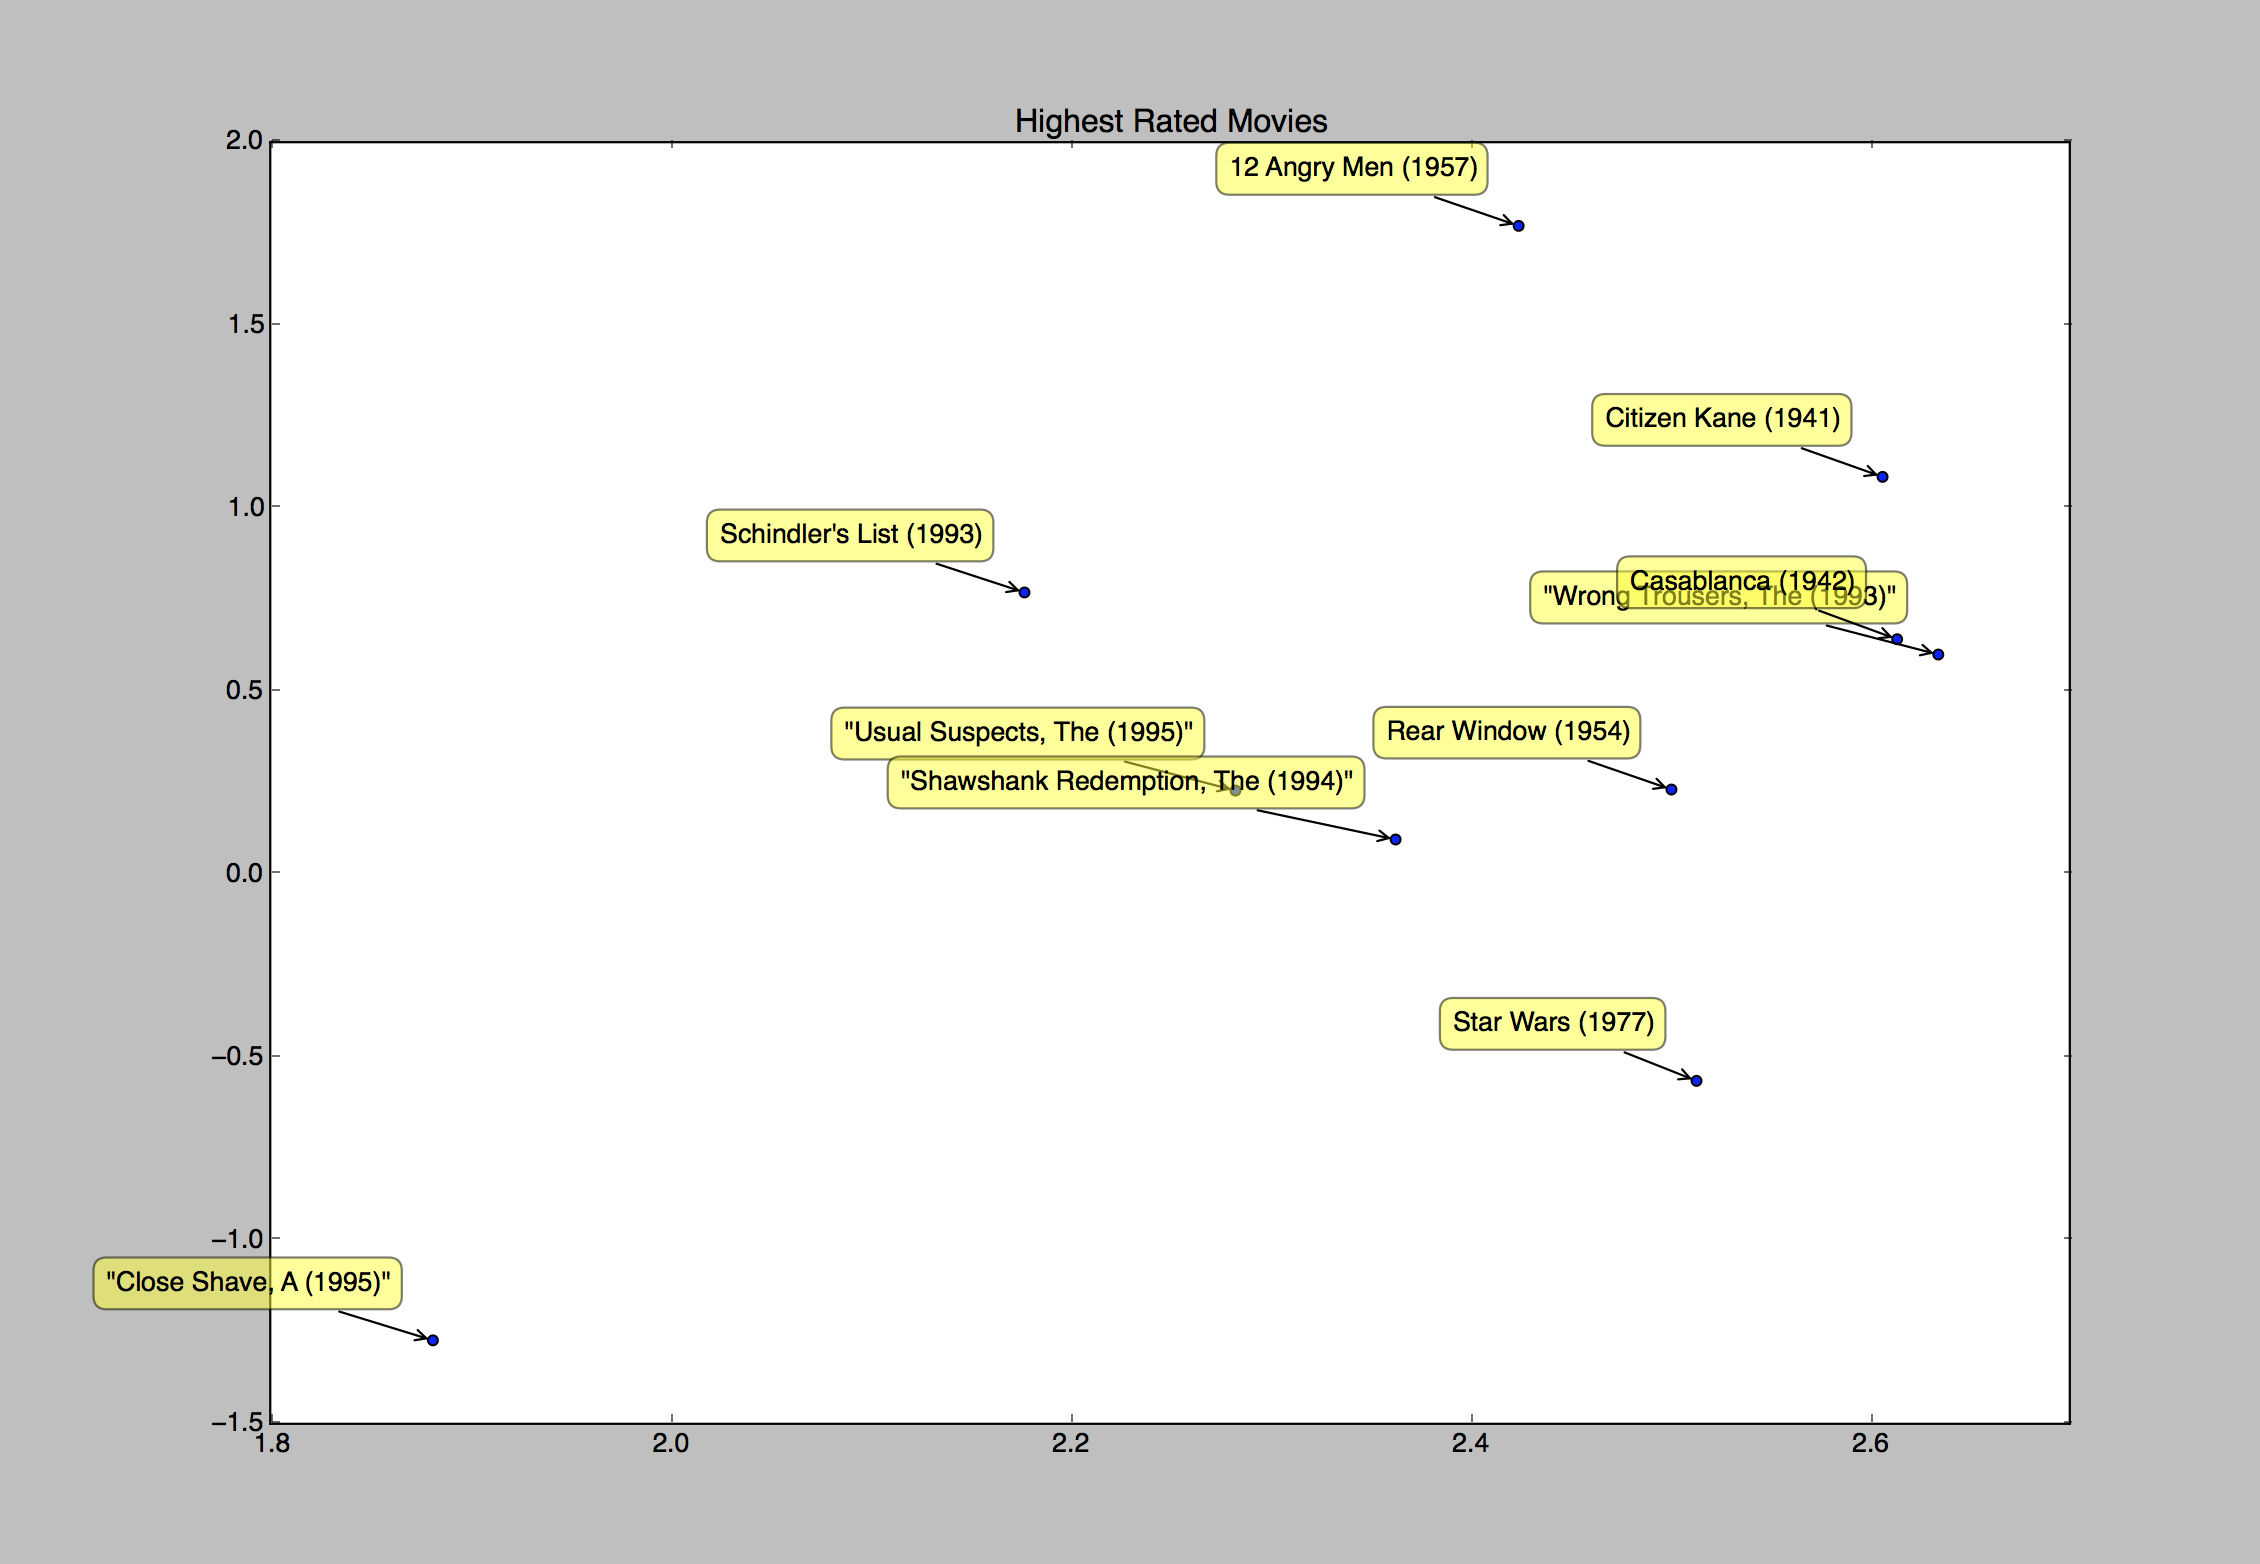
\includegraphics[width=\textwidth]{highest_2d_vis}
\caption{2D visualization of parameters for 10 best movies in the dataset.}
\end{figure}



\pagebreak

\begin{figure}[H]
\centering
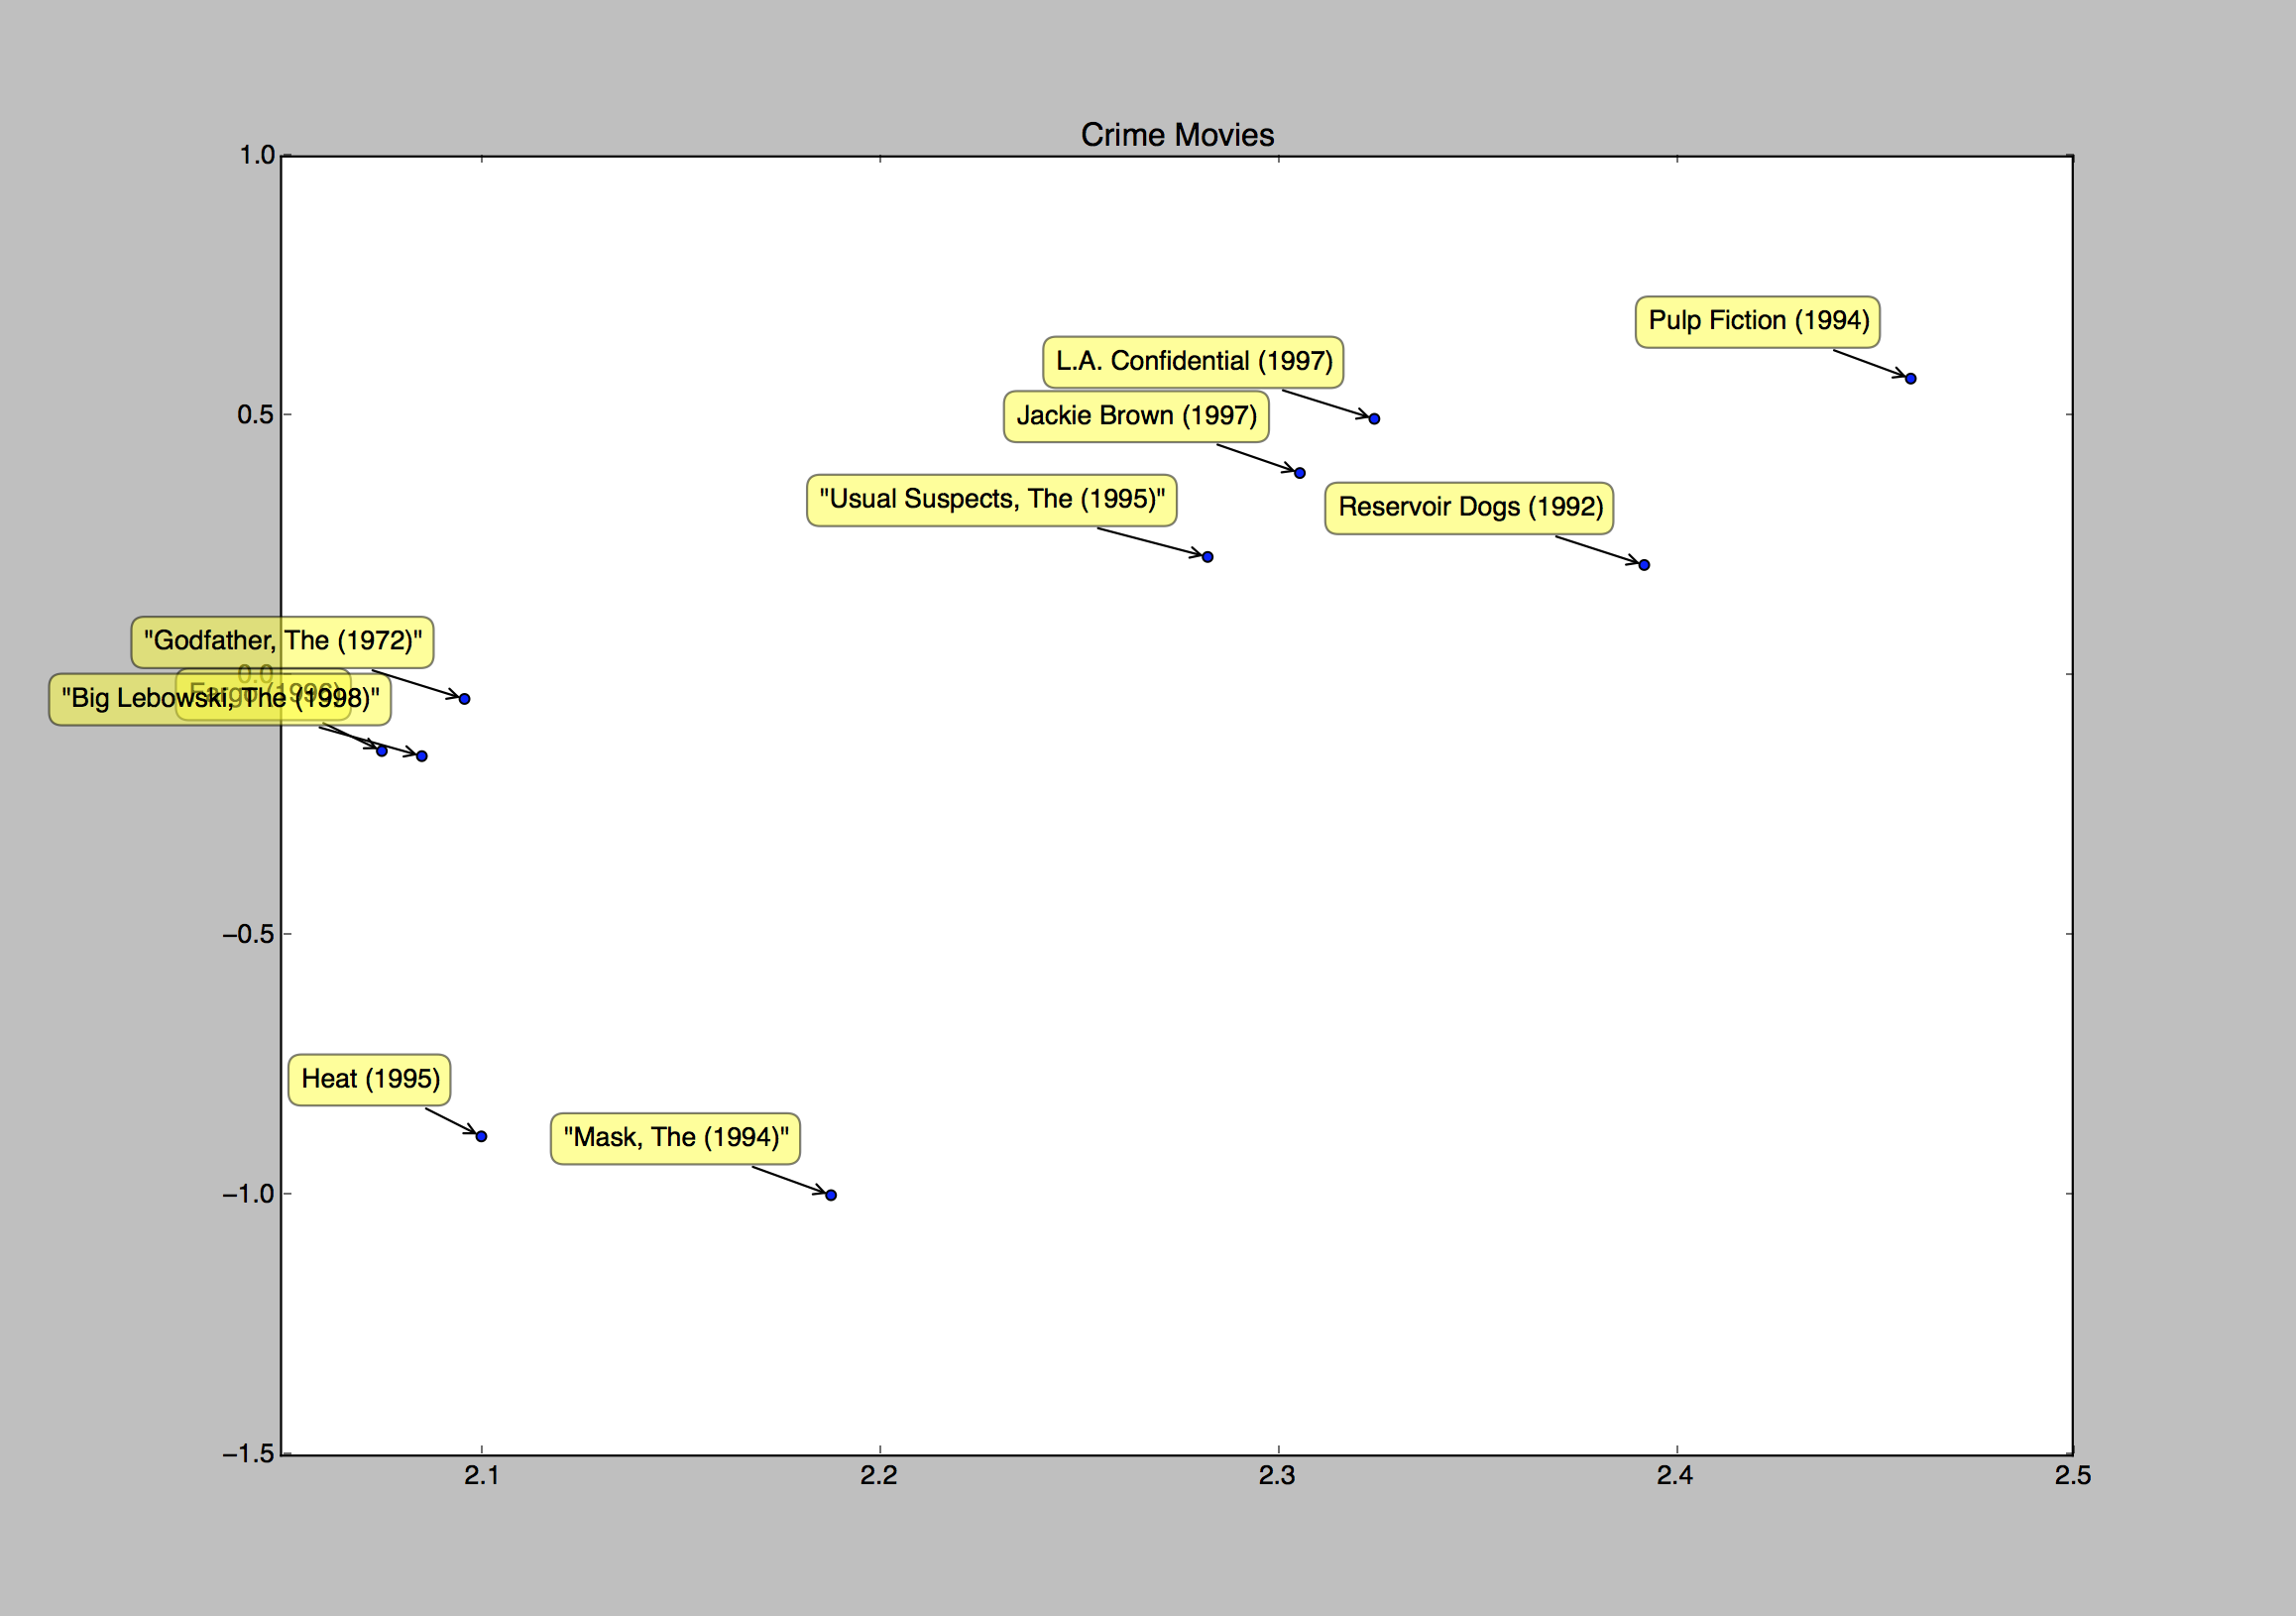
\includegraphics[width=\textwidth]{crime_2d_vis}
\caption{2D visualization of parameters for 10 crime movies in the dataset.}
\end{figure}


\pagebreak

\begin{figure}[H]
\centering
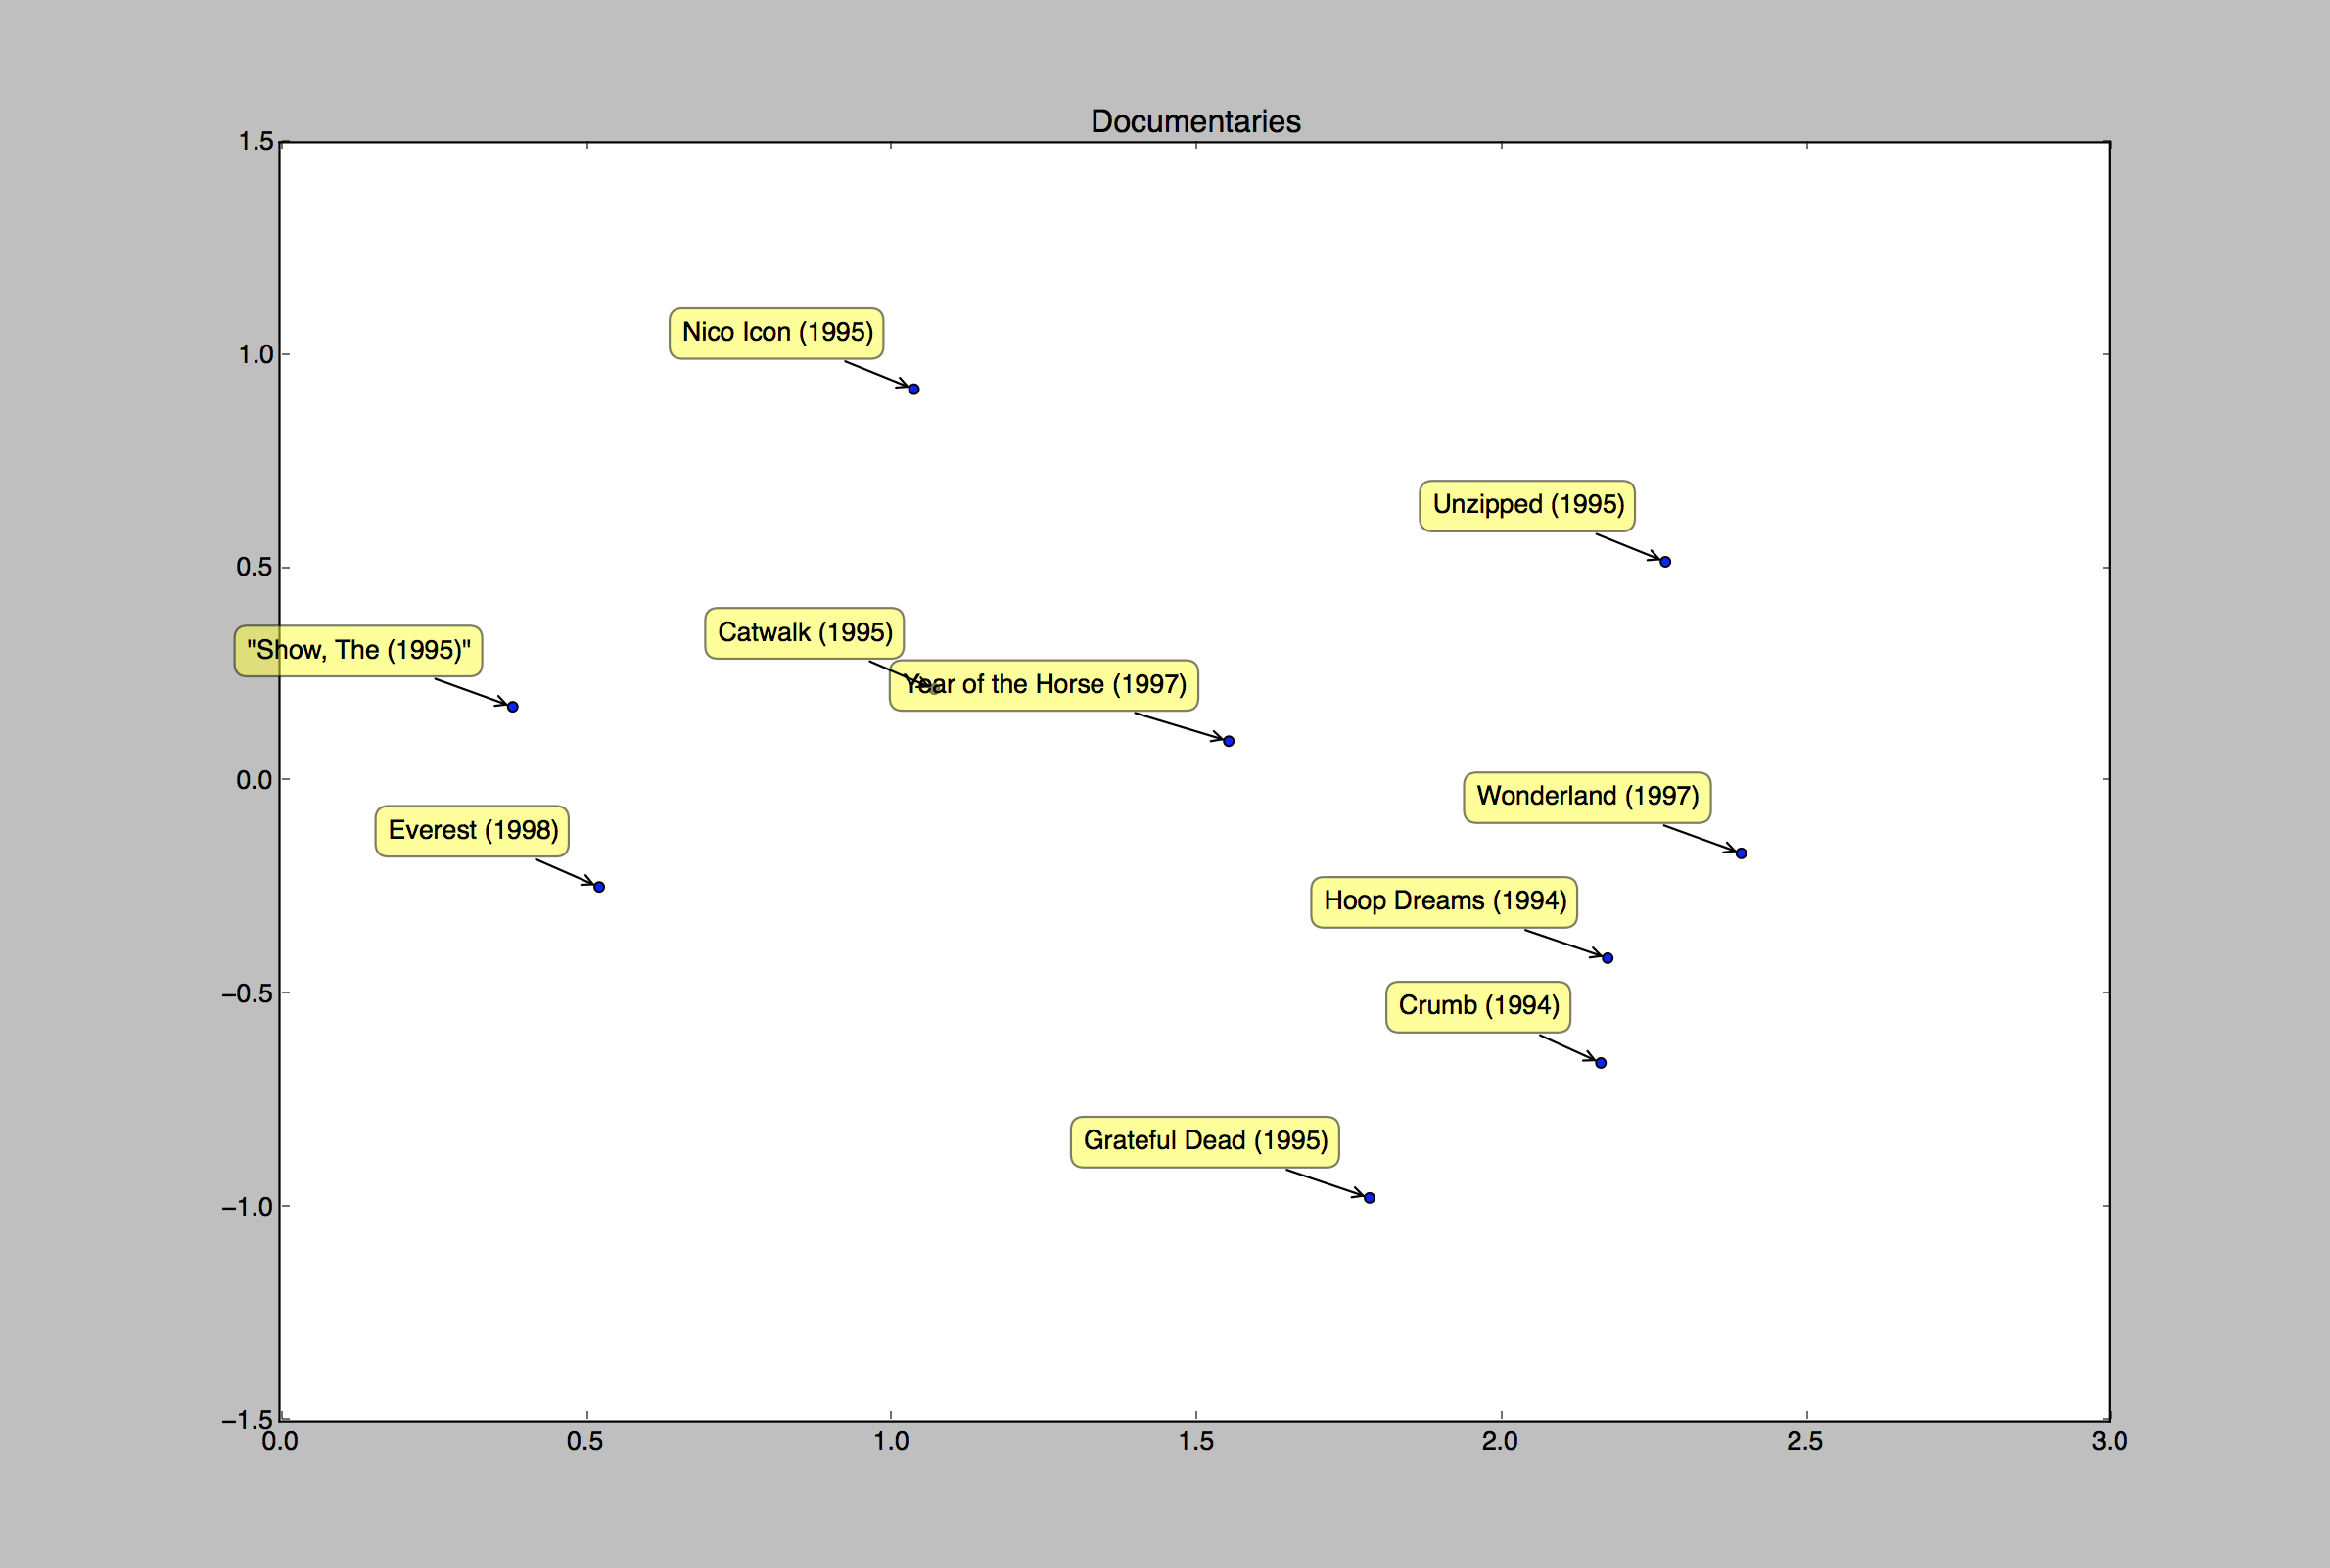
\includegraphics[width=\textwidth]{documentaries_2d_vis}
\caption{2D visualization of parameters for 10 documentary movies in the dataset.}
\end{figure}


\pagebreak

\begin{figure}[H]
\centering
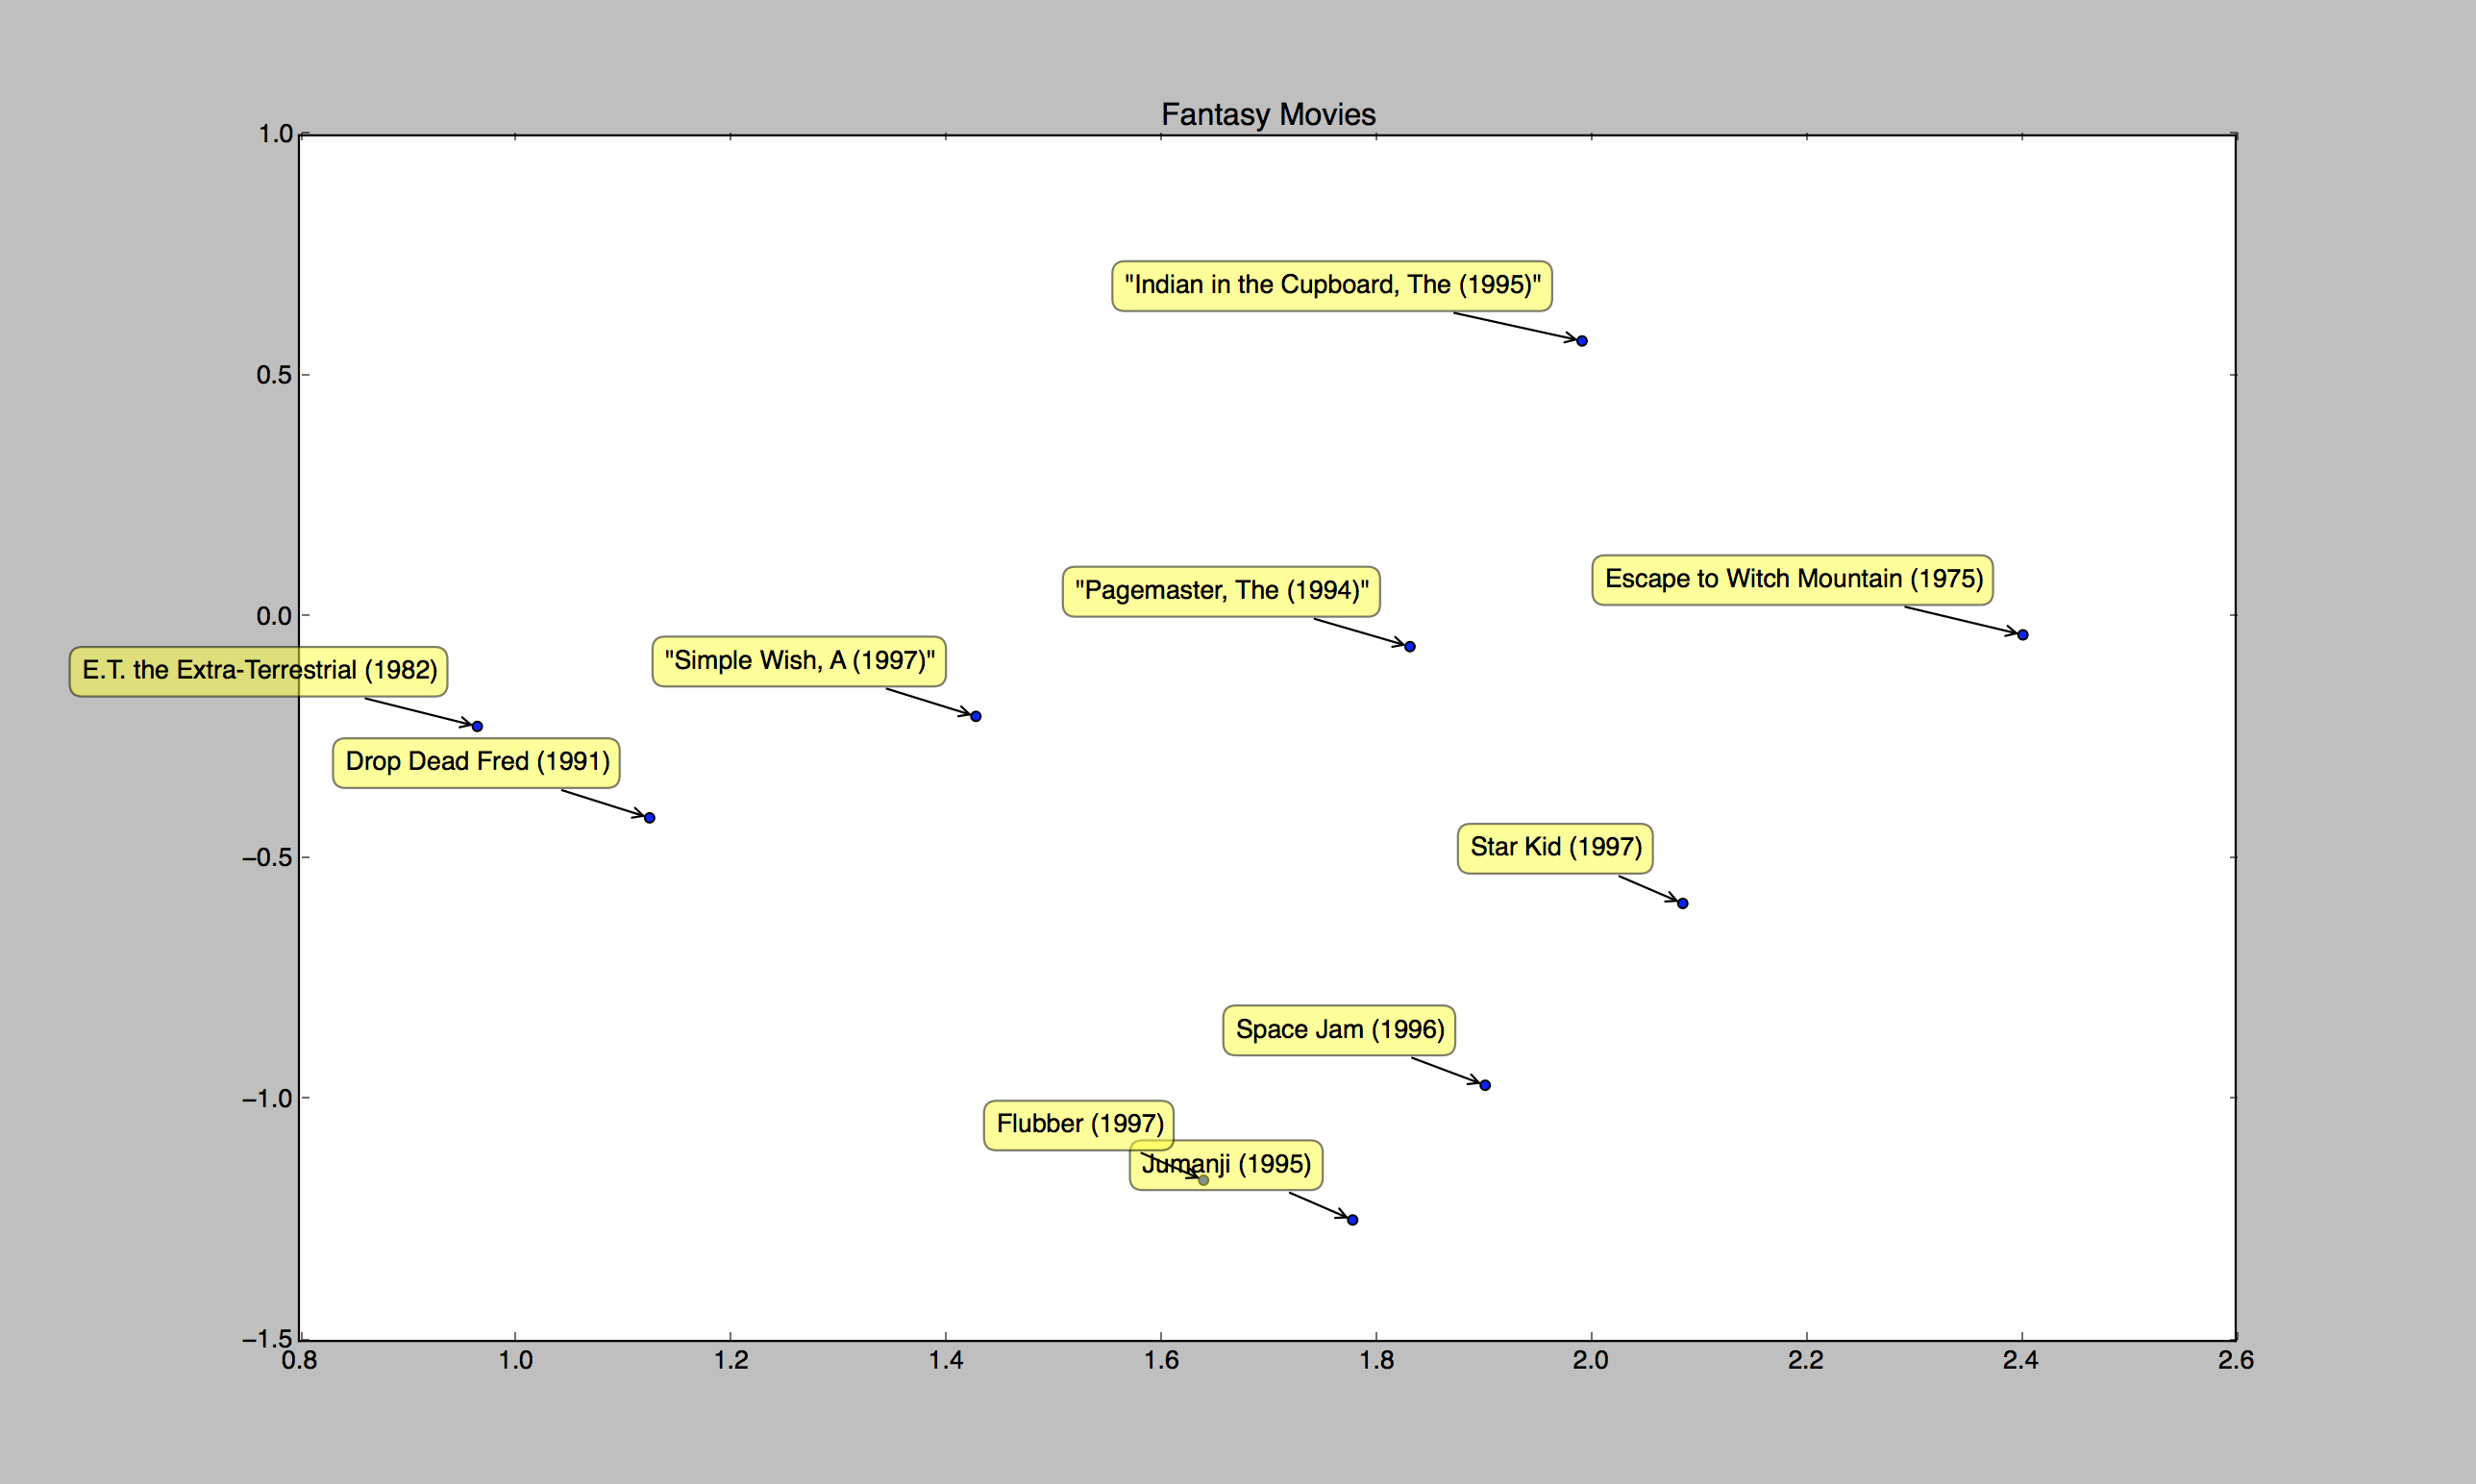
\includegraphics[width=\textwidth]{fantasy_2d_vis}
\caption{2D visualization of parameters for 10 fantasy movies in the dataset.}
\end{figure}



\begin{itemize}

    \item \boldline{What did you observe?} \\
    The goal with these plots is to determine some sort of divisive criteria
    for the two axes; something that will cause one set of people to give the
    movie a high rating while causing another set of people to give the movie
    a low rating. For the vertical axis, our best guess was that a higher Y
    value corresponded to a more serious/inaccessible movie, like a complicated
    drama or a historical movie with heavy subject matter. Conversely, a movie
    with a smaller Y value would be something with simpler, more accessible
    subject matter, like an animated kids movie, a rom-com, or an action movie.

    This trend is best illustrated in the `Highest Rated Movies' plot. At the top
    we see 12 Angry Men, a courtroom drama with lots of subtle, character-driven
    interactions. Also near the top is Schindler's List, with deals with 
    Holocaust-era Germany, and Citizen Kane, another complex mystery drama.
    Near the bottom we have A Close Shave, one of the animated Wallace and Grommit
    movies, and Star Wars, a very accessible action move.

    This trend is far from perfect though. Notice that Sleepless in Seattle,
    a fairly simple rom-com, has the same accessibility value as Schindler's List,
    which doesn't make much sense. A Close Shave and The Wrong Trousers have
    very different accessilibity values, even though they are both Wallace and
    Grommit movies and should have very similar ratings on both axes.

    We were unable to conclude anything definitive for the X axis. Notice how
    A Close Shave and The Wrong Trousers are on completely opposite sides of the X
    axis even though one is basically the sequel of the other. Similarly,
    some very different pairs have the same X value, like Casablanca and The
    Wrong Trousers, or The Godfather and The Big Lebowski. It's entirely possible
    that there is some overlap in audience of people who like both of these
    movies, but given their difference in subject matter this overlap wasn't
    apparent to us. 

    \item \boldline{How do the ratings of the best movies compare to those of the most popular movies?} \\
    The best rated movies had a wider range in Y values, while the most rated
    movies had a larger range of X values. It's hard to conclude anything too
    concrete from this. This sort of makes sense if we think of the Y axis as
    accessibility, because in order for movies to have a lot of ratings they
    have to be accessible to a lot of people, which narrows the range of possible
    Y values.

    \item \boldline{How do the ratings of the three genres you chose compare to one another?} \\

    All three genres have pretty much the same range of Y values. The crime movies
    all have very large X values, while the documentaries on average have
    much lower X values. This was the most significant observation we had for the
    X values. Perhaps a large X value corresponds to a more exciting, suspenseful
    movie, while a smaller X value corresponds to a dryer, less emotional movie.

    \item \boldline{What was expected and what was surprising from the visualizations?} \\
     We were surprised with how difficult it was to draw any concrete conclusions
    from the plots. We tried a wide range of movie combinations at different $\lambda$
    values, and no matter what we tried no obvious correlation jumped out at us,
    even with 100000 input data points. We expected these correlations would be
    a lot more apparent than they were in reality. 

\end{itemize}


\pagebreak
\section{Conclusion}
\medskip
\begin{itemize}

    \item \boldline{Briefly summarize your main observations} \\
    % Insert text here.
    Our main observations for the basic visualizations were that the ratings for many genres follow a simple unimodal distribution. Depending on the genre, this mode might be in different locations and there could also be different variances in ratings for different genres. We observed that often-rated movies don't necessarily correspond to high-rated movies: Many often-rated movies had the same distribution of ratings as the dataset as a whole. If a movie is well-liked, it can have a plurality of 5 ratings.

    Our observations from the 2d matrix factorization visualizations were a bit more ambiguous. It seems that there might be some correlations between the axes and certain movie properties such as how serious/light-hearted, or how accessible the movie was, but there were often movies that went against these trends. Perhaps there is not enough data to make these trends very consistent, since random correlations between viewers of certain types of movies could skew the results.

    \item \boldline{Did your visualizations help you to better understand the MovieLens dataset?} \\
    % Insert text here.
    In the end, we didn't learn much about the dataset that we didn't already expect. Some potential exceptions to this were the fact that popular movies aren't always rated well, and that the tone of a movie is potentially the most polarizing factor in determining whether someone likes it.

\end{itemize}



\end{document}
